\documentclass[10pt]{article}
\usepackage[margin=0.8in]{geometry}
\usepackage{amsmath,amssymb,booktabs,enumitem,xcolor,graphicx,float,microtype,tabularx}
\usepackage[most]{tcolorbox}
\usepackage[colorlinks=true,linkcolor=blue!50!black,urlcolor=blue!50!black]{hyperref}
\setlength{\parskip}{3pt}\setlength{\parindent}{0pt}
\setlist{leftmargin=*,itemsep=1pt,topsep=2pt}
\graphicspath{{figures/}}
\newcolumntype{Y}{>{\raggedright\arraybackslash}X}
\newcommand{\E}{\mathbb{E}}
\newtcolorbox{key}[1]{colback=blue!3,colframe=blue!40!black,fonttitle=\bfseries,title=#1,boxrule=0.6pt,arc=2pt}
\newtcolorbox{res}[1]{colback=green!3,colframe=green!40!black,fonttitle=\bfseries,title=#1,boxrule=0.6pt,arc=2pt}
\newtcolorbox{open}[1]{colback=orange!4,colframe=orange!60!black,fonttitle=\bfseries,title=#1,boxrule=0.6pt,arc=2pt}

\title{\textbf{Reward Shaping Is Noise Shaping,\\ and a Law for the Accuracy--Diversity Frontier of RLVR}\\[4pt]\large Project report: what is established, what is open, what is running}
\author{Mohamed Ayman}
\date{October 23, 2026}

\begin{document}
\maketitle
\vspace{-10pt}

\begin{key}{The project in five points}
\begin{enumerate}
\item \textbf{Question.} RLVR methods that change how answers are scored claim more diversity (pass@$k$), but they are compared at the same training step. Is the diversity real?
\item \textbf{Diagnosis (established).} Every correctness-only scoring rule pushes the model in the same expected direction and differs only in per-question weight and noise; noise sets the \emph{speed} along one accuracy--diversity curve. At matched accuracy, the rules coincide on two model families, and zero-mean noise alone reproduces NSR's behaviour.
\item \textbf{Methods (so far small).} Replaying successes, inside RL, gives about $+1$ point of pass@16 at matched accuracy. A warm start on base-model successes and groups of 32 rollouts go far beyond Dr.\ GRPO's accuracy range, so they cannot yet be compared at matched accuracy.
\item \textbf{New: a frontier law.} Starting only from the base model's per-question success counts, a two-parameter model of per-question log-odds learning predicts pass@16 within 1--2 points for nine further training rules, a second model family, and a larger answer budget (pre-registered, prospective). It fails after a warm start.
\item \textbf{Status.} Independent review (Codex): the diagnosis alone about 5/10; with the law passing its prospective tests about 7/10; with a method that improves the frontier across scales about 8/10. The long-run test of the law, the 2026-methods audit, and the method pilot are running.
\end{enumerate}
\end{key}

\section{Setting and terms}
Qwen2.5-Math-1.5B (main) and OLMo-2-1B (replication), MATH training questions, 150 RL steps of 16 questions $\times$ 8 answers, AdamW $10^{-6}$, answers up to 512 tokens; evaluation on 511 held-out MATH test problems (answer keys audited) with 32 samples per problem.
\begin{center}\small
\begin{tabularx}{\linewidth}{@{}p{0.2\linewidth}Y@{}}
\toprule
pass@1 / pass@$k$ & accuracy / chance that at least one of $k$ answers is right (``diversity'')\\
Dr.\ GRPO (B) & advantage $A=r-\bar r$; the reference method\\
PSR / NSR & reward right answers only ($A=r$) / penalize wrong answers only ($A=r-1$)\\
Matched accuracy & pass@16 compared at the same pass@1, interpolated along B's trajectory (and its temperature envelope)\\
\bottomrule
\end{tabularx}
\end{center}

\section{The diagnosis (finished)}
\textbf{Theory.} For any rule that scores answers by correctness alone, with $p$ a question's success rate,
$\E g=c(p)\,\nabla p$ and $\E\|g\|^2=F_1D_1(p)+F_0D_0(p)+\|\nabla p\|^2X(p)$:
a rule can only reweight questions ($c$) and change the noise ($D_1,D_0$). Wrong answers carry most of it (2--3$\times$ larger squared gradients, measured on both families). At matched pass@1, pass@$k=\E_x[1-(1-p_x)^k]$, so diversity at equal accuracy is how evenly success is spread across questions.

\begin{figure}[H]\centering
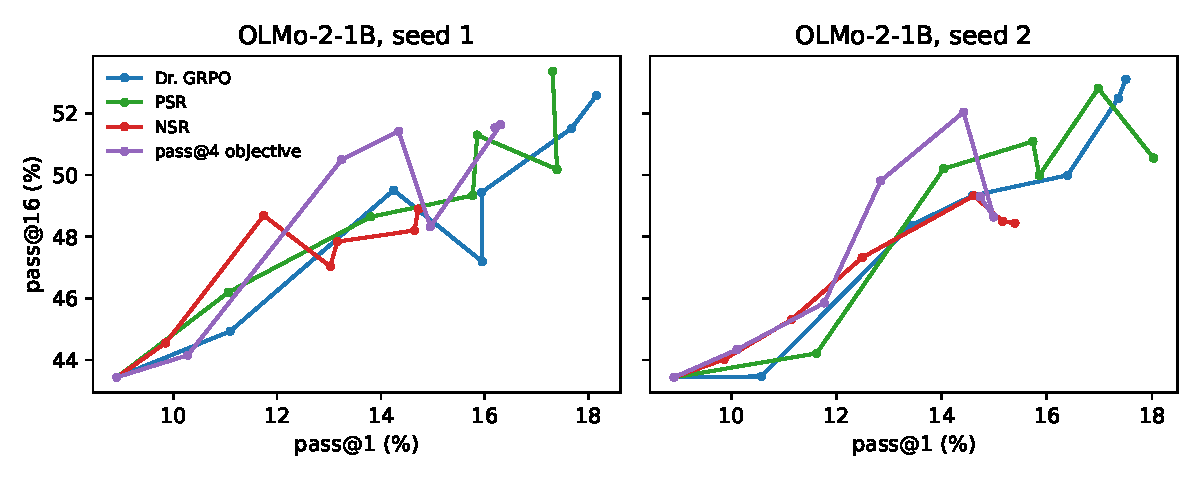
\includegraphics[width=0.48\linewidth]{olmo_curves.pdf}\hfill
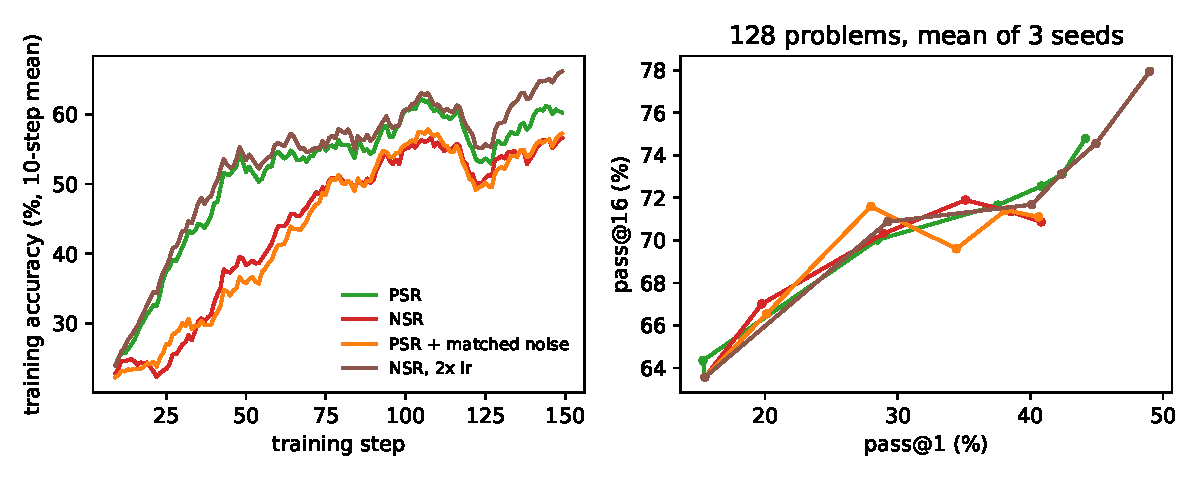
\includegraphics[width=0.48\linewidth]{noise_test.pdf}
\caption{Left: OLMo-2-1B, five rules on one accuracy--diversity curve. Right: Qwen; PSR plus zero-mean noise of NSR's size learns as slowly as NSR, and all lie on one curve.}
\end{figure}

\begin{res}{Established findings}
\begin{enumerate}
\item \textbf{One curve.} PSR, NSR, five constant baselines, the NSR paper's own implementation and a pass@4 objective all move along one curve on Qwen; on OLMo, NSR minus PSR at matched accuracy is $-0.30$, 90\% $[-1.28,+0.77]$ (equivalent within $\pm2$).
\item \textbf{Noise is the cause.} Adding zero-mean random-sign noise of NSR's size to PSR makes it as slow as NSR (speed $\phi=-0.11$ $[-0.22,-0.05]$; NSR $=0$, PSR $=1$); NSR at twice the learning rate recovers. With Adam, noise misdirects rather than shrinks steps.
\item \textbf{Not a temperature effect.} RL barely changes entropy on fixed text ($1.081\to1.064$) but cuts it 3--4$\times$ on its own samples; a late checkpoint sampled hotter does not beat the training curve ($-1.42$, 90\% $[-2.19,-0.68]$).
\item \textbf{Popular fixes stay on the curve:} entropy bonus, adaptive entropy and entropy floors (which stop learning), and the published unlikeliness reward ($+0.14$).
\end{enumerate}
\end{res}

\section{Trying to move the curve}
\begin{center}\small
\begin{tabularx}{\linewidth}{@{}Y p{0.25\linewidth} p{0.2\linewidth}@{}}
\toprule
Method (3 seeds, 511 problems unless noted) & pass@16 at matched accuracy & Status\\
\midrule
Reward shaping, entropy control, unlikeliness, pass@$k$ objective & $\approx 0$ & finished\\
Coverage-weighted replay of own successes (Pre-reg.\ 12) & $+1.19$ $[+0.54,+1.79]$ & finished; below $+2$\\
Base-seeded replay, Option A (Pre-reg.\ 14) & $+1.02$ $[+0.23,+1.68]$; pass@1 $-5.4$ at step 150 & finished (main arms)\\
Annealed replay; MaxRL with group completion (pilot, 1 seed, validation) & $+1.30$; $+1.12$; both pass@1 $-6.5$ & pilot, interim\\
Group completion; prefix-guided rollouts (pilot) & -- & being evaluated\\
Warm start: fine-tune on base successes, then Dr.\ GRPO & beyond B's range (pass@1 52.5 vs 44.1) & not comparable yet\\
Groups of 32 rollouts (4$\times$ samples) & beyond B's range (pass@1 52.5) & 2 of 3 seeds\\
\bottomrule
\end{tabularx}
\end{center}

\begin{figure}[H]\centering
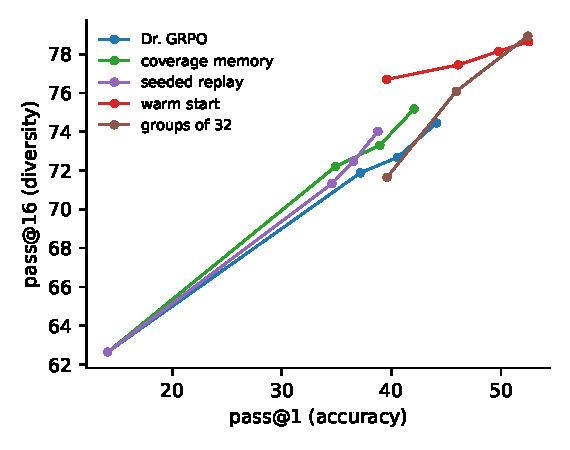
\includegraphics[width=0.46\linewidth]{frontier_qwen.pdf}\hfill
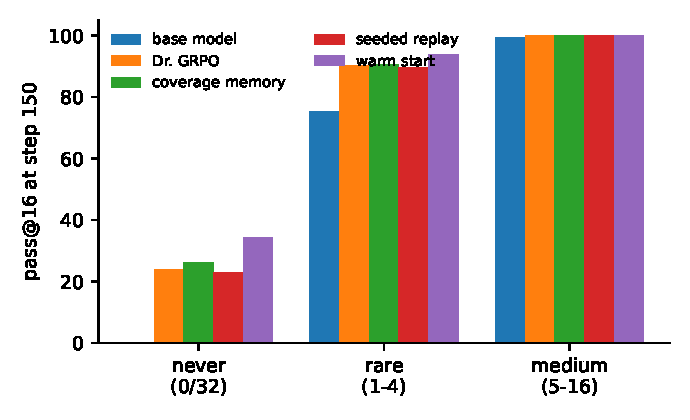
\includegraphics[width=0.52\linewidth]{strata.pdf}
\caption{Left: the Qwen frontier (seed means). The warm start and groups of 32 end at the same point (pass@1 52.5, pass@16 about 79), beyond anything Dr.\ GRPO reaches in 150 steps. Right: pass@16 at step 150 by how often the base model solved each problem; the warm start's gain sits on problems the base never solves (24 $\to$ 34).}
\end{figure}

\textbf{The 512-token budget matters.} At 512 tokens, 48\% of Dr.\ GRPO's sampled answers at step 150 are truncated. Re-evaluated at 1,024 tokens (Check 16, partial), Dr.\ GRPO's step-150 pass@1 is 57.7 (vs 44.6) and pass@16 88.4 (vs 75.2), with 15.5\% truncated; the warm start reaches 63.8 and 89.7 (4.9\% truncated). Every absolute number in the project depends on the budget; the comparisons are made within one budget, and the law (Section 4) was checked at both.

\section{The frontier law (Pre-registration 17)}
\begin{key}{The law}
Each question's log-odds start at the base model's empirical-Bayes estimate $\theta_x(0)=\log\frac{c_x+a}{n-c_x+b}$ and grow as
$\dot\theta_x=p_x(1-p_x)+\tau\,\overline{p(1-p)}$:
own-signal logistic learning plus a uniform transfer term. A checkpoint is placed where the predicted mean success equals its observed pass@1; the law then predicts the rest of the distribution (pass@$k$, difficulty strata, per-question counts). Two parameters: progress $t$ (matched) and $\tau$ (fitted once on Dr.\ GRPO, $\tau=-0.20$, then frozen).
\end{key}

\begin{figure}[H]\centering
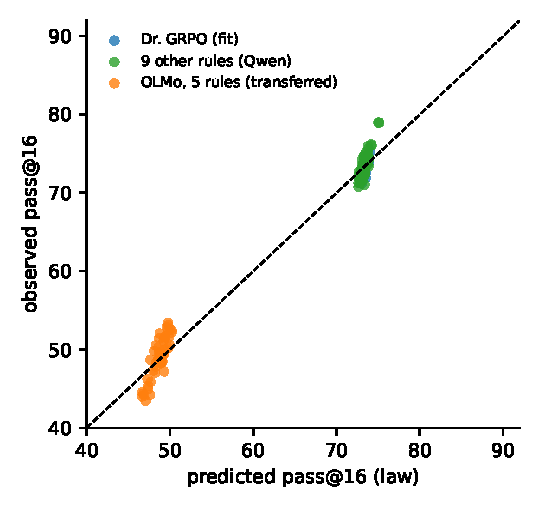
\includegraphics[width=0.42\linewidth]{law_fit.pdf}
\caption{Predicted against observed pass@16. Blue: Dr.\ GRPO (fit). Green: nine further rules on Qwen. Orange: OLMo, five rules, $\tau$ transferred from Qwen without refitting.}
\end{figure}

\begin{center}\small
\begin{tabularx}{\linewidth}{@{}Y c c c c@{}}
\toprule
Test set (law frozen before each) & ckpts & RMSE: law / unif. / affine & verdict & beats affine\\
\midrule
Fit: Dr.\ GRPO (in-sample) & 9 & 1.06 / 21.3 / 1.28 & -- & 9/9\\
T1: nine other rules on Qwen & 56 & \textbf{1.21} / 20.1 / 2.45 & supported & 54/56\\
T4: OLMo, $\tau$ from Qwen & 50 & \textbf{1.90} / 9.9 / 12.6 & supported & 50/50\\
T5: 1,024-token budget & 4 & \textbf{0.85} / 11.5 / 1.27 & supported & 4/4\\
T2: warm start, from its own step-0 counts & 9 & 3.56 / 9.0 / 8.0 & falsified & 9/9\\
T3: 450-step Dr.\ GRPO (beyond the fitted range) & -- & running & -- & --\\
\bottomrule
\end{tabularx}
\end{center}
``Uniform'': every question's log-odds shift by the same amount; ``affine'': $\theta'=\alpha+\beta\theta$ with $\beta$ fitted on the same data. ``Beats affine'': higher per-question likelihood of the observed counts.

\textbf{Reading.} From a base model, the frontier of every rule we ran, on two families and two budgets, is predicted by the base difficulty distribution plus near-independent per-question learning; rules differ in how far along the trajectory they get. Diversity collapse is a rich-get-richer effect: a uniform improvement would lift never-solved problems to about 70--80 pass@16, the observed value is 24. Two levers can move this frontier: the starting distribution (information about rare questions) and transfer between questions. \textbf{The exception}: after a warm start, RL lifts never-solved problems about 12 points less than the law predicts (refitted $\tau=-0.65$ to $-0.70$ in all seeds, against $-0.20$ from the base model): fine-tuning changes the dynamics, not only the starting point.

\textbf{Against the law's extended frontier} (the law from base counts, used beyond Dr.\ GRPO's range), the warm start is $+3.3$ to $+3.6$ points above at every checkpoint and groups of 32 reaches $+3.9$ at step 150; Dr.\ GRPO itself drifts from $-1.2$ to $+0.5$. Whether the warm start is genuinely above Dr.\ GRPO's curve depends on how the law extrapolates, which the 450-step run (T3) measures.

\section{Does training transfer to rarely solved questions? (Check 17, partial)}
For 395 held-out problems, the margin between the likelihood of the base model's correct and wrong answers (style cancels). Seed 8 of Dr.\ GRPO: the margin rises by $+0.025$ nats per token on both rarely solved and medium problems by step 150; the warm start (seed 9) is $+0.039$ above the base on rare problems right after fine-tuning and $+0.049$ by step 150. Interim reading: Dr.\ GRPO does transfer to rare problems about as much as to medium ones, so the ``little transfer'' premise is not supported in this seed; four of six lanes are still running.

\section{Position in the 2026 literature}
\begin{itemize}
\item \textbf{Unpublished (ours):} noise sets speed along one curve; NSR on PSR's curve on two families; the noise-injection causal test; the matched-accuracy protocol; temperature does not beat the curve; a prospective law for the frontier from base counts. No 2026 method paper compares at matched accuracy.
\item \textbf{Published:} ``same direction, per-question weight'' (Davis \& Recht 2025; Heckel et al.\ 2026); base-seeded replay (TAR, Oct.\ 2026); nearly our coverage weight (BBG); replay and off-policy rescue of all-wrong groups (LSPO, LUFFY, ExGRPO); transfer-driven curricula (TAC, GradAlign); per-prompt GRPO recurrences (Mroueh 2025); the Matthew effect (NGU); ``RLVR is a Kernel'', which argues base success does not determine post-RL success and is the strongest challenge to the law.
\end{itemize}

\section{Assessment and next steps}
\begin{open}{Open questions and what decides them}
\begin{enumerate}
\item \textbf{Does the law extrapolate?} T3 (450-step Dr.\ GRPO, seed 13 on AWS; 14 and 15 on Tamia) and the deep base sampling of the 309 hardest problems (which identifies the sign of $\tau$).
\item \textbf{Is the warm start (and groups of 32) above the frontier, or only faster along it?} Decided by T3's extended reference and by Check 16 at 1,024 tokens.
\item \textbf{Which method?} The pilot's group completion and prefix-guided rollouts (being evaluated); the law suggests a method that allocates demonstration acquisition where it predicts stalls, compared with random allocation and the warm start at equal compute (needs its own novelty check).
\item \textbf{The 2026 audit:} TAR (3 seeds trained, being evaluated), BBG, MaxRL, W-REINFORCE (partly trained) at matched accuracy, and against the law.
\end{enumerate}
\end{open}
\textbf{Paper shape if T3 passes:} the diagnosis (one curve, noise sets speed, matched accuracy) $\to$ the law (the frontier predicted from base difficulty; why reward shaping cannot move it; the warm-start exception) $\to$ the matched-accuracy audit of 2026 methods $\to$ a method derived from the law. Independent review estimates 7/10 for this shape if the prospective tests pass.

\appendix
\section{Experiment ledger}
\begin{center}\scriptsize
\begin{tabularx}{\linewidth}{@{}p{0.07\linewidth} Y p{0.36\linewidth}@{}}
\toprule
& Question & Outcome\\
\midrule
P1--3 & Scale down wrong answers; collection rules at equal cost; noise inside training & noise formula fits; the optimal collection rule moves faster along the curve\\
P4 & PSR vs NSR, clean on-policy & NSR 6.4$\times$ noisier, slower, same pass@64: separation not reproduced\\
P5 & NSR vs PSR at matched accuracy & no extra diversity ($-2.1$, $-0.2$)\\
P6 & The NSR paper's implementation & not recreated; clipping active on 26--28\% of NSR's steps\\
P7 & Same mean, graded noise (baselines) & speed follows predicted noise (rank correlation 0.9--0.97)\\
P8 & pass@4 objective; reasoning graded & curve fixed ($+1.6$, $+0.2$); reasoning-checked diversity equal\\
P9 & OLMo-2-1B replication & one curve: NSR$-$PSR $-0.30$ $[-1.28,+0.77]$\\
P10 & Is noise the cause? & yes: PSR + noise as slow as NSR\\
P11 & Is the curve a temperature effect? & no ($-1.42$ $[-2.19,-0.68]$)\\
P12 & Coverage-weighted replay & $+1.19$ $[+0.54,+1.79]$, average agreement\\
P14 & Base-seeded replay and controls & $+1.02$; slower; warm start far ahead\\
P15 & 2026 methods at matched accuracy (TAR, BBG, MaxRL, W-REINFORCE) & running\\
P16 & Push mechanisms inside RL (pilot) & interim: replay variants $\approx+1.2$ but 6.5 points less accurate\\
P17 & The frontier law & supported on T1, T4, T5; falsified on T2; T3 running\\
Check 16 & 512 vs 1,024 tokens & all numbers rise at 1,024; comparisons pending\\
Check 17 & Transfer to rare problems & partial: Dr.\ GRPO transfers to rare as to medium\\
\bottomrule
\end{tabularx}
\end{center}
All experiments were pre-registered and reviewed by an independent model before launch; the records are the pre-registration, results and check files in \texttt{experiments/training/}.
\end{document}
